%===============================================================================
\chapter{Strongly Correlated Electrons: The Hubbard Model}
\label{ch:hubbard}
%===============================================================================

The Hubbard model captures the essential physics of strongly correlated electron systems, where the interplay between electron kinetic energy and on-site repulsion produces a rich phase diagram. This chapter applies the geometric RG framework of Part I to a condensed matter system where strong correlations challenge perturbative methods and reveal the full power of RG thinking. The functional RG provides a non-perturbative approach that interpolates between weak and strong coupling.

The scale hierarchy compares the bandwidth $W \sim zt$ to the interaction strength $U$. Coarse-graining can proceed from weak coupling (integrating out high-energy particle-hole excitations) or strong coupling (integrating out doubly occupied states). Theory space includes the ratio $U/t$, the filling, and temperature. The beta functions are computed via perturbative or functional methods. Fixed-point analysis reveals multiple competing phases: Fermi liquid, Mott insulator, superconductor, and possibly strange metal.

\marginnote{The Hubbard model was introduced independently by Hubbard, Gutzwiller, and Kanamori in 1963 to explain magnetism and metal-insulator transitions.}

%-------------------------------------------------------------------------------
\section{The Hubbard Hamiltonian}
\label{sec:hubbard_hamiltonian}
%-------------------------------------------------------------------------------

The Hubbard model describes electrons hopping on a lattice with an on-site repulsion:
\begin{equation}
H = -t \sum_{\langle i,j \rangle, \sigma} (c^\dagger_{i\sigma} c_{j\sigma} + \text{h.c.}) + U \sum_i n_{i\uparrow} n_{i\downarrow}
\label{eq:hubbard}
\end{equation}
where $c^\dagger_{i\sigma}$ creates an electron with spin $\sigma$ at site $i$, $n_{i\sigma} = c^\dagger_{i\sigma} c_{i\sigma}$ is the number operator, $t$ is the hopping amplitude, and $U > 0$ is the on-site Coulomb repulsion.

\subsection{Scale Identification}

Following Step 1 of the recipe, we identify the scales. The bandwidth $W \sim zt$ (where $z$ is the coordination number) sets the kinetic energy scale, characterizing how much energy an electron gains by delocalizing across the lattice. The interaction $U$ is the potential energy scale, the cost of putting two electrons on the same site. The dimensionless coupling $u = U/W$ measures the relative strength of interactions: when $u \ll 1$ kinetic energy dominates and electrons form a Fermi liquid, while when $u \gg 1$ interactions dominate and electrons localize into a Mott insulator.

The scale parameter can be taken as the energy cutoff $\Lambda$ or temperature $T$. As we lower $\Lambda$ or $T$, the effective coupling can flow to strong or weak values depending on the bare parameters and dimensionality.

\marginnote{The ratio $U/t$ controls whether electrons behave as itinerant metals or localized moments.}

%-------------------------------------------------------------------------------
\section{Limiting Cases}
\label{sec:hubbard_limits}
%-------------------------------------------------------------------------------

The physics depends dramatically on the ratio $U/t$ and the electron filling.

\subsection{Weak Coupling: $U \ll t$}

For small $U$, electrons form a Fermi liquid with renormalized parameters. Standard perturbation theory in $U/t$ applies, and the system is metallic.

\subsection{Strong Coupling: $U \gg t$}

For large $U$, double occupancy is energetically suppressed. At half-filling (one electron per site on average), the system becomes a Mott insulator with localized spins. The effective low-energy theory is the Heisenberg antiferromagnet:
\begin{equation}
H_{\text{eff}} = J \sum_{\langle i,j \rangle} \mathbf{S}_i \cdot \mathbf{S}_j
\label{eq:heisenberg}
\end{equation}
with exchange coupling $J = 4t^2/U$.

\subsection{The Mott Transition}

As $U/t$ increases from zero, the system undergoes a metal-insulator transition (Mott transition) at some critical value $(U/t)_c$. This is a quantum phase transition driven by the competition between kinetic and potential energy.

%-------------------------------------------------------------------------------
\section{RG for the Hubbard Model}
\label{sec:hubbard_rg}
%-------------------------------------------------------------------------------

Several RG approaches have been developed for the Hubbard model.

\subsection{Weak Coupling RG}

For $U \ll t$, perturbative RG can be developed around the free electron fixed point. The beta function for the interaction strength depends on the dimensionality and band structure.

In one dimension with a linear spectrum near the Fermi points, the RG equations for the coupling constants $g_i$ (characterizing different scattering processes) take the form:
\begin{align}
\frac{dg_1}{d\ell} &= -g_1^2 + \cdots, \label{eq:hubbard_g1}\\
\frac{dg_2}{d\ell} &= -2g_1 g_2 + \cdots, \label{eq:hubbard_g2}
\end{align}
where $\ell = \ln(\Lambda_0/\Lambda)$ is the logarithmic scale.

\marginnote{The 1D Hubbard model is exactly solvable by the Bethe ansatz, providing a benchmark for RG calculations.}

\subsection{Strong Coupling RG}

For $U \gg t$, one starts from the atomic limit and treats hopping as a perturbation. The RG generates effective interactions at lower energy scales.

The key insight is that high-energy virtual excitations (creating double occupancies) are integrated out, generating the superexchange coupling $J$ and other effective interactions.

%-------------------------------------------------------------------------------
\section{Fixed Points and Phase Diagram}
\label{sec:hubbard_fixed}
%-------------------------------------------------------------------------------

Applying the framework of Chapter~\ref{ch:fixed_points}:

\subsection{One Dimension}

In 1D at half-filling, the repulsive Hubbard model flows toward a Mott insulating fixed point for any $U > 0$. The fixed point is described by a Luttinger liquid with gapless spin excitations governed by the effective Heisenberg antiferromagnetic coupling, and gapped charge excitations reflecting the Mott gap that prevents charge transport. Away from half-filling, the system remains metallic but as a Luttinger liquid rather than a Fermi liquid, with power-law correlations rather than quasiparticle excitations.

\subsection{Two Dimensions}

The 2D Hubbard model is believed to describe high-temperature superconductivity in the cuprates. The RG analysis reveals a complex phase diagram with multiple competing phases. At half-filling and sufficiently strong coupling $U > U_c$, the system forms an antiferromagnetic Mott insulator. Upon doping away from half-filling, d-wave superconductivity may emerge from the pairing of electrons mediated by antiferromagnetic fluctuations. At weak coupling, the system exhibits Fermi liquid behavior with well-defined quasiparticles.

The phase diagram involves multiple competing fixed points, and no single analytical method captures all regimes. Numerical methods including quantum Monte Carlo, dynamical mean-field theory, and tensor networks complement the analytical RG, each providing insight into different corners of parameter space.

\marginnote{The 2D Hubbard model remains one of the great unsolved problems in condensed matter physics.}

\subsection{Infinite Dimensions}

In the limit $d \to \infty$ (with proper scaling of $t$), the Hubbard model becomes exactly solvable via dynamical mean-field theory (DMFT). This provides a nonperturbative benchmark for understanding the Mott transition. A sharp first-order Mott transition occurs at $(U/W)_c \approx 1.5$, with a metal-insulator coexistence region where both phases are locally stable. The crossover from itinerant to localized behavior can be traced continuously as $U/W$ increases, with spectral weight transferring from coherent quasiparticle peaks to incoherent Hubbard bands.

\subsection{The Mott Transition as RG Flow}

\marginnote{The Mott transition exemplifies how RG flows can connect qualitatively different fixed points: itinerant electrons $\to$ localized moments.}

Following Sethna's perspective on metal-insulator transitions, we can understand the Mott transition geometrically as a flow in theory space. The key insight is that the quasiparticle weight $Z$---the discontinuity in the momentum distribution at the Fermi surface---serves as a natural coordinate on theory space:

\begin{itemize}
\item \textbf{Fermi liquid ($Z > 0$)}: Well-defined quasiparticles with renormalized mass $m^*/m = 1/Z$.
\item \textbf{Mott insulator ($Z = 0$)}: Quasiparticles cease to exist; charge is localized.
\end{itemize}

The RG flow drives $Z$ under coarse-graining:
\begin{equation}
\frac{dZ}{d\ell} = \beta_Z(U/t, n, T)
\end{equation}

At weak coupling, $Z$ flows toward a finite value (Fermi liquid fixed point). At strong coupling, $Z$ flows to zero (Mott fixed point). The critical surface $Z = 0$ is an \textbf{attractor} for the strong-coupling phase.

\begin{workedbox}[Box 14.2: Order Parameters for the Mott Transition]
The Mott transition is subtle because there is no broken symmetry in the conventional sense. Following Sethna's classification of phase transitions:

\textbf{What is the order parameter?} Several candidates:
\begin{enumerate}
\item \textbf{Quasiparticle weight $Z$}: Vanishes in the Mott insulator.
\item \textbf{Charge compressibility $\kappa = \partial n/\partial \mu$}: Vanishes as the charge gap opens.
\item \textbf{Double occupancy $D = \langle n_\uparrow n_\downarrow \rangle$}: Suppressed in the Mott insulator.
\end{enumerate}

\textbf{What is the symmetry?} Unlike conventional transitions, no symmetry is broken. The Mott transition is a \textbf{topological} phase transition---the Fermi surface changes topology (from a finite surface to a point, then to nothing).

\textbf{RG interpretation}: The transition is between two distinct universality classes. The Fermi liquid and Mott insulator fixed points have different relevant operators and different low-energy excitations. The critical point is either:
\begin{itemize}
\item First order (as in DMFT): two coexisting fixed points
\item Continuous (in some models): an unstable fixed point at the transition
\end{itemize}

This exemplifies Sethna's point that phase transitions need not involve broken symmetry---the RG provides the unifying framework.
\end{workedbox}

The Brinkman-Rice scenario provides a mean-field picture of the Mott transition. As $U$ increases, the effective mass diverges:
\begin{equation}
\frac{m^*}{m} = \frac{1}{Z} = \frac{1}{1 - (U/U_c)^2} \to \infty \quad \text{as } U \to U_c^-
\end{equation}

This is analogous to critical slowing down: near the transition, low-energy excitations become very ``heavy'' (slow). In the RG language, the correlation time diverges as the system approaches the critical surface.

The connection to our geometric framework is direct:
\begin{itemize}
\item \textbf{Theory space}: Coordinates $(U/t, n, T, Z, \ldots)$
\item \textbf{Fixed points}: Fermi liquid (finite $Z$), Mott insulator ($Z = 0$), superconductor
\item \textbf{Relevant/irrelevant}: At the Fermi liquid fixed point, $U$ is marginally irrelevant in $d > 1$
\item \textbf{Critical surface}: The Mott transition separates basins of attraction
\end{itemize}

%-------------------------------------------------------------------------------
\section{Functional RG Approach}
\label{sec:hubbard_frg}
%-------------------------------------------------------------------------------

The functional renormalization group provides a systematic nonperturbative framework for the Hubbard model. This approach, based on an exact flow equation for the effective action, allows interpolation between weak and strong coupling.

\subsection{The Effective Action}

Define the generating functional for connected Green's functions $W[J]$ and its Legendre transform, the effective action $\Gamma[\phi]$. Introducing a regulator $R_\Lambda$ that suppresses modes below the scale $\Lambda$:
\begin{equation}
\Gamma_\Lambda[\phi] = \sup_J \left( J \cdot \phi - W_\Lambda[J] \right) - \Delta S_\Lambda[\phi]
\end{equation}
where $\Delta S_\Lambda$ is the regulator contribution.

\subsection{The Flow Equation}

The exact RG equation for $\Gamma_\Lambda$ is:
\begin{equation}
\frac{\partial \Gamma_\Lambda}{\partial \Lambda} = \frac{1}{2} \text{Tr} \left[ \left( \Gamma_\Lambda^{(2)} + R_\Lambda \right)^{-1} \frac{\partial R_\Lambda}{\partial \Lambda} \right]
\label{eq:wetterich_hubbard}
\end{equation}
where $\Gamma_\Lambda^{(2)}$ is the second functional derivative of the effective action.

\marginnote{The functional RG provides a nonperturbative framework valid at any coupling strength.}

\subsection{Truncation and Results}

Practical calculations require truncating the effective action to a finite number of coupling constants. Common truncations include the static four-point vertex, which captures magnetic and pairing instabilities; the frequency-dependent vertex, which captures dynamic correlations; and self-energy effects, which capture spectral weight transfer between coherent and incoherent excitations. More sophisticated truncations include momentum dependence and higher-order vertices.

The functional RG has successfully predicted several key features of the Hubbard model phase diagram. Antiferromagnetic order emerges at half-filling when the nesting of the Fermi surface enhances magnetic susceptibility. Upon doping, d-wave pairing can arise from antiferromagnetic fluctuations acting as a pairing glue. Pseudogap behavior in the underdoped regime, where spectral weight is suppressed near the Fermi level even above the superconducting transition, also emerges naturally from the functional RG flow.

%-------------------------------------------------------------------------------
\section{Connection to the Anharmonic Oscillator}
\label{sec:hubbard_anharmonic}
%-------------------------------------------------------------------------------

There is a deep connection between the Hubbard model and the anharmonic oscillator of the Prologue.

\subsection{Path Integral Representation}

In the coherent state path integral, the Hubbard model becomes:
\begin{equation}
Z = \int \mathcal{D}[\bar{c}, c] \, e^{-S[\bar{c}, c]}
\end{equation}
with action containing quadratic (kinetic) and quartic (interaction) terms.

This has the same structure as the $\phi^4$ theory, with fermionic (Grassmann) fields instead of bosonic ones. The RG analysis proceeds similarly, with complications from the Fermi surface geometry.

\subsection{Local vs. Itinerant Physics}

The competition between $t$ (promoting delocalization) and $U$ (promoting localization) mirrors the competition between kinetic and potential energy in the anharmonic oscillator. The RG identifies which physics dominates at low energies.

%-------------------------------------------------------------------------------
\section{Emergent Phenomena}
\label{sec:hubbard_emergent}
%-------------------------------------------------------------------------------

The Hubbard model exhibits emergent phenomena that arise from the RG flow.

\subsection{Antiferromagnetism}

At half-filling with moderate $U$, antiferromagnetic order emerges below a N\'{e}el temperature $T_N$. The RG shows that antiferromagnetic fluctuations are relevant perturbations that flow to strong coupling.

\subsection{Superconductivity}

Upon doping, the antiferromagnetic fluctuations can mediate an effective attractive interaction between electrons, potentially leading to superconductivity. The RG identifies the pairing symmetry (typically d-wave in 2D cuprates).

\marginnote{The mechanism of high-temperature superconductivity remains one of the outstanding problems in physics.}

\subsection{Strange Metal}

In certain parameter regimes, the Hubbard model may flow toward a ``strange metal'' fixed point characterized by non-Fermi liquid behavior: linear-in-$T$ resistivity, anomalous scaling of transport properties, and absence of well-defined quasiparticles.

%-------------------------------------------------------------------------------
\section{Connection to the Geometric Framework}
\label{sec:hubbard_geometry}
%-------------------------------------------------------------------------------

We now connect the Hubbard model to the geometric framework of Part I.

\subsection{Theory Space}

The theory space for the Hubbard model includes the interaction strength $U/t$, the electron filling $n$ (from empty to half-filled to fully occupied), temperature $T$ or equivalently the energy scale $\Lambda$, and in extended models, longer-range interactions and additional orbitals. The RG flow traces a trajectory through this high-dimensional space, with different regions flowing to different fixed points.

\subsection{Fixed Points and Phases}

Different phases correspond to different fixed points in theory space. The Fermi liquid is described by a free fermion fixed point with renormalized parameters including the quasiparticle mass and Landau interaction parameters. The Mott insulator corresponds to a strong coupling fixed point with localized spins and a charge gap. The superconductor is a BCS-type fixed point with Cooper pairing. A strange metal phase, if it exists, would correspond to a non-Fermi liquid fixed point with anomalous scaling and no well-defined quasiparticles. Phase transitions are crossovers between basins of attraction of these different fixed points.

\subsection{Stability Analysis}

At each fixed point, the stability matrix of Chapter~\ref{ch:fixed_points} determines the fate of perturbations. Relevant perturbations destabilize the phase and drive transitions to other fixed points. Irrelevant perturbations flow to zero and do not affect the long-distance physics. Marginal perturbations require higher-order analysis to determine their ultimate behavior.

For the Fermi liquid fixed point in dimensions $d > 1$, forward scattering is marginal, corresponding to the renormalization of Landau parameters. BCS pairing is marginally relevant at zero temperature in the presence of an attractive interaction, explaining why arbitrarily weak attraction leads to superconductivity.

\subsection{The Metric on Theory Space}

While less developed than in CFT, a metric on the coupling space can be defined from susceptibilities:
\begin{equation}
G_{ij} = \frac{\partial^2 F}{\partial g^i \partial g^j}
\end{equation}
where $F$ is the free energy density and $g^i$ are the couplings.

This metric diverges at phase transitions (critical points), reflecting the singular behavior of the thermodynamic potentials.

%-------------------------------------------------------------------------------
\section*{Exercises}
\addcontentsline{toc}{section}{Exercises}
%-------------------------------------------------------------------------------

\begin{enumerate}
\item \textbf{Strong coupling expansion.} In the limit $U \gg t$, derive the effective Heisenberg Hamiltonian~\eqref{eq:heisenberg} using second-order perturbation theory in $t/U$.
\begin{enumerate}
\item Show that the superexchange coupling is $J = 4t^2/U$.
\item Explain why the effective interaction is antiferromagnetic ($J > 0$).
\item Discuss what happens at third order in $t/U$.
\end{enumerate}

\item \textbf{Fermi liquid stability.} For the 2D Hubbard model at weak coupling, the system is a Fermi liquid.
\begin{enumerate}
\item What is the quasiparticle residue $Z$ and how does it depend on $U/t$?
\item At what coupling strength do you expect Fermi liquid theory to break down?
\item Discuss the role of nesting in destabilizing the Fermi liquid.
\end{enumerate}

\item \textbf{Mott transition.} At half-filling, the Hubbard model undergoes a metal-insulator transition.
\begin{enumerate}
\item In the Brinkman-Rice picture, how does the quasiparticle weight $Z$ vanish as $U \to U_c$?
\item In DMFT, the transition can be first-order. Sketch the phase diagram in the $(U/t, T)$ plane.
\item Discuss the critical exponents associated with the Mott transition in mean-field theory.
\end{enumerate}

\item \textbf{Functional RG.} Consider the Wetterich equation~\eqref{eq:wetterich_hubbard} for the Hubbard model.
\begin{enumerate}
\item Explain the role of the regulator $R_\Lambda$.
\item What is the initial condition for $\Gamma_\Lambda$ at $\Lambda = \Lambda_0$?
\item How does the effective four-fermion interaction flow under the RG?
\end{enumerate}

\item \textbf{(Challenge) d-wave superconductivity.} In the 2D Hubbard model near half-filling:
\begin{enumerate}
\item Explain how antiferromagnetic fluctuations can mediate an effective attractive interaction.
\item Why is d-wave pairing favored over s-wave?
\item Relate the superconducting $T_c$ to the antiferromagnetic exchange coupling $J$.
\end{enumerate}

\item \textbf{Quasiparticle breakdown.} (Inspired by Sethna) The quasiparticle weight $Z$ provides a coordinate on theory space.
\begin{enumerate}
\item In a Fermi liquid, $Z$ is the jump in the momentum distribution at $k_F$. Explain why $0 < Z \leq 1$ and what $Z = 1$ corresponds to.
\item The effective mass satisfies $m^*/m = 1/Z$. As $Z \to 0$, how does the density of states at the Fermi level behave?
\item In the Brinkman-Rice scenario, $Z = 1 - (U/U_c)^2$. Show this implies $m^* \to \infty$ as $U \to U_c$.
\item Interpret this divergence in terms of critical slowing down near a fixed point.
\end{enumerate}

\item \textbf{RG flow in the Hubbard model.} (Inspired by Sethna) Consider the theory space with coordinates $(U/t, T, n - 1)$ where $n$ is the filling.
\begin{enumerate}
\item Sketch the RG flow diagram in the $(U/t, T)$ plane at half-filling ($n = 1$). Identify the Fermi liquid, Mott insulator, and antiferromagnetic fixed points.
\item How does doping ($n \neq 1$) change the flow? Why does the Mott insulator become unstable to doping?
\item In 1D, the Mott insulator is stable for any $U > 0$ at half-filling. What is special about 1D that prevents a metal-insulator transition?
\item The functional RG provides a controlled interpolation between weak and strong coupling. Sketch how the effective interaction vertex evolves under the RG flow from $\Lambda_0$ to $\Lambda = 0$.
\end{enumerate}

\item \textbf{Connection to percolation.} (Inspired by Sethna) Metal-insulator transitions can also occur due to disorder (Anderson localization) or classical percolation.
\begin{enumerate}
\item In classical percolation, the conductivity vanishes when the network of conducting bonds disconnects. What is the order parameter?
\item Compare the Mott transition (interaction-driven) to Anderson localization (disorder-driven). Both give insulating behavior, but how do they differ in their RG fixed points?
\item The metal-insulator transition in doped semiconductors involves both disorder and interactions. Discuss how the RG might handle this ``Mott-Anderson'' transition.
\end{enumerate}
\end{enumerate}

%-------------------------------------------------------------------------------
\subsection*{Solutions}
%-------------------------------------------------------------------------------

\begin{solutionbox}{Exercise 14.1: Strong Coupling Expansion}
\textbf{(a) Superexchange coupling $J = 4t^2/U$.}

Consider two adjacent sites with one electron each. In the atomic limit ($t=0$), the ground state has energy $E_0 = 0$ (no double occupancy).

Second-order perturbation theory in $t$:
\begin{equation}
E^{(2)} = \sum_n \frac{|\langle n|H_t|0\rangle|^2}{E_0 - E_n}
\end{equation}

The hopping Hamiltonian $H_t = -t\sum_{\langle ij\rangle,\sigma}(c^\dagger_{i\sigma}c_{j\sigma} + \text{h.c.})$ can create a virtual doubly-occupied state with energy $E_n = U$.

For antiparallel spins $|\uparrow_1\downarrow_2\rangle$:
\begin{equation}
E^{(2)}_{\text{AF}} = -\frac{2t^2}{U} \quad \text{(electron can hop either direction)}
\end{equation}

For parallel spins $|\uparrow_1\uparrow_2\rangle$: $E^{(2)}_{\text{F}} = 0$ (Pauli exclusion blocks hopping).

The energy difference favors antiparallel alignment:
\begin{equation}
\Delta E = E^{(2)}_{\text{AF}} - E^{(2)}_{\text{F}} = -\frac{2t^2}{U}
\end{equation}

This can be written as $\mathbf{S}_1 \cdot \mathbf{S}_2 = -3/4$ for singlet, $+1/4$ for triplet, giving:
\begin{equation}
H_{\text{eff}} = J\mathbf{S}_1 \cdot \mathbf{S}_2 + \text{const}, \quad \boxed{J = \frac{4t^2}{U}}
\end{equation}

\textbf{(b) Why antiferromagnetic ($J > 0$).}

With our convention $H = J\sum \mathbf{S}_i \cdot \mathbf{S}_j$:
\begin{itemize}
\item $J > 0$ favors $\mathbf{S}_i \cdot \mathbf{S}_j < 0$ (antiparallel spins)
\item Physical reason: antiparallel spins allow virtual hopping (kinetic energy gain)
\item Parallel spins are blocked by Pauli exclusion (no kinetic energy gain)
\end{itemize}

\textbf{(c) Third order in $t/U$.}

At third order, three-site terms appear:
\begin{equation}
H^{(3)} \sim \frac{t^3}{U^2}\sum_{\langle ijk\rangle}(\mathbf{S}_i \times \mathbf{S}_j)\cdot\mathbf{S}_k
\end{equation}

This is a chiral spin interaction that breaks time-reversal on frustrated lattices. It's relevant for spin liquids and topological phases.
\end{solutionbox}

\begin{solutionbox}{Exercise 14.2: Fermi Liquid Stability}
\textbf{(a) Quasiparticle residue $Z$.}

The quasiparticle residue is:
\begin{equation}
Z = \left(1 - \frac{\partial\Sigma(\omega)}{\partial\omega}\Big|_{\omega=0}\right)^{-1}
\end{equation}

At weak coupling (first-order in $U$), $\Sigma$ has no frequency dependence, so $Z = 1$.

At second order:
\begin{equation}
Z \approx 1 - \frac{U^2}{W^2}f(n) + O(U^4)
\end{equation}
where $f(n)$ depends on filling $n$ and band structure.

\textbf{(b) Breakdown of Fermi liquid.}

Fermi liquid theory breaks down when:
\begin{enumerate}
\item $Z \to 0$: quasiparticles lose coherence
\item Interaction energy $\sim U$ becomes comparable to bandwidth $W$
\item At half-filling: Mott transition near $U_c \sim W$
\end{enumerate}

For the 2D square lattice: $U_c/t \approx 8$ from DMFT, so $U_c \sim W$.

\textbf{(c) Role of nesting.}

At half-filling on a square lattice, the Fermi surface has perfect nesting: $\epsilon_{k+Q} = -\epsilon_k$ for $Q = (\pi,\pi)$.

Nesting enhances:
\begin{itemize}
\item Particle-hole susceptibility $\chi(Q) \sim \ln^2(W/T)$ (logarithmically divergent)
\item Antiferromagnetic correlations
\item Instability toward SDW (spin density wave) order
\end{itemize}

Even weak $U$ can destabilize the Fermi liquid when nesting is perfect.
\end{solutionbox}

\begin{solutionbox}{Exercise 14.3: Mott Transition}
\textbf{(a) Brinkman-Rice picture.}

In the Gutzwiller approximation, the quasiparticle weight:
\begin{equation}
Z = \frac{1 - (U/U_c)^2}{1 + (U/U_c)^2} \quad\text{(simplified form)}
\end{equation}

Near the transition:
\begin{equation}
\boxed{Z \sim (U_c - U)^\alpha \to 0 \quad\text{as } U \to U_c^-}
\end{equation}

with $\alpha = 1$ in mean-field. The effective mass $m^*/m = 1/Z \to \infty$.

\textbf{(b) DMFT phase diagram.}

In DMFT, the Mott transition at half-filling is first-order at $T < T_c$:

\begin{center}
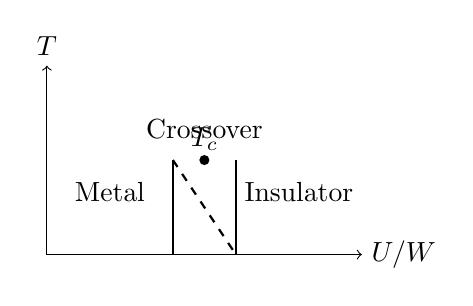
\begin{tikzpicture}[scale=0.8]
\draw[->] (0,0) -- (5,0) node[right] {$U/W$};
\draw[->] (0,0) -- (0,3) node[above] {$T$};
\draw[thick] (2,0) -- (2,1.5);
\draw[thick,dashed] (2,1.5) -- (3,0);
\draw[thick] (3,0) -- (3,1.5);
\node at (1,1) {Metal};
\node at (4,1) {Insulator};
\node at (2.5,2) {Crossover};
\filldraw (2.5,1.5) circle (2pt) node[above] {$T_c$};
\end{tikzpicture}
\end{center}

Key features:
\begin{itemize}
\item First-order transition at $T < T_c$ (coexistence region)
\item Critical endpoint at $T_c$
\item Crossover for $T > T_c$
\end{itemize}

\textbf{(c) Critical exponents (mean-field).}

At the critical endpoint, mean-field exponents:
\begin{itemize}
\item Order parameter: $\Delta \sim |U - U_c|^{1/2}$ ($\beta = 1/2$)
\item Susceptibility: $\chi \sim |U - U_c|^{-1}$ ($\gamma = 1$)
\item Correlation length: $\xi \sim |U - U_c|^{-1/2}$ ($\nu = 1/2$)
\end{itemize}

These satisfy mean-field scaling relations $\gamma = 2\beta$, $\nu = \beta/d$ for $d > d_c = 4$.
\end{solutionbox}

\begin{solutionbox}{Exercise 14.4: Functional RG}
\textbf{(a) Role of regulator $R_\Lambda$.}

The regulator $R_\Lambda$ in the Wetterich equation:
\begin{equation}
\partial_\Lambda\Gamma_\Lambda = \frac{1}{2}\text{Tr}\left[(\Gamma^{(2)}_\Lambda + R_\Lambda)^{-1}\partial_\Lambda R_\Lambda\right]
\end{equation}

serves to:
\begin{enumerate}
\item Suppress modes with $|k| < \Lambda$ (IR regularization)
\item Interpolate smoothly between $\Gamma_{\Lambda_0} = S$ (bare action) and $\Gamma_0 = \Gamma$ (full effective action)
\item Ensure the flow is well-defined at each scale
\end{enumerate}

Common choice: $R_\Lambda(k) = (k^2 - \Lambda^2)\theta(\Lambda^2 - k^2)$ (Litim regulator).

\textbf{(b) Initial condition.}

At $\Lambda = \Lambda_0$ (UV cutoff):
\begin{equation}
\boxed{\Gamma_{\Lambda_0}[\psi] = S[\psi]}
\end{equation}

The effective action equals the bare action because no modes have been integrated out yet.

\textbf{(c) Four-fermion flow.}

The effective four-fermion interaction $U_\Lambda$ flows according to:
\begin{equation}
\partial_\Lambda U_\Lambda = -\frac{U_\Lambda^2}{\Lambda^2}(\chi_{\text{ph}} + \chi_{\text{pp}}) + \cdots
\end{equation}

where $\chi_{\text{ph}}$ and $\chi_{\text{pp}}$ are particle-hole and particle-particle bubbles.

Key physics:
\begin{itemize}
\item Particle-hole channel enhances magnetic correlations
\item Particle-particle channel can generate pairing
\item Competition determines the ground state
\end{itemize}
\end{solutionbox}

\begin{solutionbox}{Exercise 14.5: d-Wave Superconductivity (Challenge)}
\textbf{(a) Antiferromagnetic fluctuations as glue.}

Near half-filling, AF fluctuations create a spin susceptibility peaked at $Q = (\pi,\pi)$:
\begin{equation}
\chi_s(q) \approx \frac{\chi_0}{1 + \xi^2(q-Q)^2}
\end{equation}

The effective electron-electron interaction mediated by spin fluctuations:
\begin{equation}
V_{\text{eff}}(k,k') = U^2\chi_s(k-k')
\end{equation}

This is \textit{repulsive} in the s-wave channel but can be \textit{attractive} in the d-wave channel when properly averaged over the Fermi surface.

\textbf{(b) Why d-wave is favored.}

The gap function $\Delta_k$ must satisfy the gap equation:
\begin{equation}
\Delta_k = -\sum_{k'} V_{\text{eff}}(k,k')\frac{\Delta_{k'}}{2E_{k'}}
\end{equation}

For d-wave: $\Delta_k = \Delta_0(\cos k_x - \cos k_y)$

The d-wave symmetry:
\begin{itemize}
\item Changes sign under $90^\circ$ rotation: $\Delta(k_x,k_y) = -\Delta(k_y,-k_x)$
\item Nodes along $(k_x = \pm k_y)$ directions
\item Sign change allows repulsive $V_{\text{eff}}$ to become attractive in the pairing channel
\end{itemize}

\textbf{(c) $T_c$ and $J$ relation.}

From spin fluctuation theory:
\begin{equation}
k_B T_c \sim J \cdot e^{-1/\lambda}
\end{equation}

where $\lambda \sim J\rho_F$ is the dimensionless coupling and $\rho_F$ is the density of states.

More quantitatively:
\begin{equation}
\boxed{T_c \sim 0.01-0.1 \times J}
\end{equation}

For cuprates with $J \sim 1500$ K, this gives $T_c \sim 15-150$ K, consistent with observed values.
\end{solutionbox}

\begin{solutionbox}{Exercise 14.6: Quasiparticle Breakdown}
\textbf{(a) Interpretation of $Z$.}

In a non-interacting system, the momentum distribution $n_k$ has a sharp jump of magnitude 1 at $k_F$. Interactions smear this jump, but in a Fermi liquid the jump survives with reduced magnitude $Z < 1$.

$Z = 1$: Non-interacting electrons (free Fermi gas).

$0 < Z < 1$: Interacting Fermi liquid with well-defined quasiparticles.

$Z = 0$: No quasiparticles; the one-particle spectral function has no coherent peak.

\textbf{(b) Density of states behavior.}

The quasiparticle density of states at the Fermi level:
\begin{equation}
N^*(E_F) = Z \cdot N_0(E_F) \cdot \frac{m^*}{m}
\end{equation}

Since $m^*/m = 1/Z$, we get $N^*(E_F) = N_0(E_F)$---the Fermi liquid DOS is unchanged! However, this DOS is spread over quasiparticle states, not bare electrons.

As $Z \to 0$, the quasiparticle spectral weight vanishes and the coherent peak broadens into an incoherent background.

\textbf{(c) Brinkman-Rice scenario.}

Given $Z = 1 - (U/U_c)^2$:
\begin{equation}
m^* = \frac{m}{Z} = \frac{m}{1 - (U/U_c)^2} \xrightarrow{U \to U_c^-} \infty
\end{equation}

The effective mass diverges at the transition, meaning electrons become infinitely heavy---they localize.

\textbf{(d) Critical slowing down interpretation.}

The characteristic timescale for quasiparticle dynamics is:
\begin{equation}
\tau \sim \hbar/(\epsilon_F Z) \sim 1/Z \to \infty
\end{equation}

As $U \to U_c$, quasiparticles become infinitely slow---they ``freeze.'' This is exactly analogous to critical slowing down near a continuous phase transition, where relaxation times diverge as the correlation length diverges.

In RG terms: the system is approaching an unstable fixed point (the Mott critical point). Near this fixed point, the relevant operator (deviation from criticality) has a small eigenvalue, leading to slow dynamics.
\end{solutionbox}

\begin{solutionbox}{Exercise 14.7: RG Flow in the Hubbard Model}
\textbf{(a) Flow diagram at half-filling.}

At half-filling, the phase diagram in $(U/t, T)$ shows:
\begin{itemize}
\item \textbf{High $T$}: Paramagnetic metal for all $U/t$
\item \textbf{Low $T$, small $U/t$}: Fermi liquid (weakly renormalized quasiparticles)
\item \textbf{Low $T$, large $U/t$}: Antiferromagnetic Mott insulator
\item \textbf{Intermediate}: Metal-insulator crossover (or first-order transition in DMFT)
\end{itemize}

RG flows:
\begin{itemize}
\item From high $T$, flows downward toward the zero-$T$ fixed points
\item Weak coupling: flows to Fermi liquid fixed point
\item Strong coupling: flows to Mott/AF fixed point
\item Critical surface separates the basins of attraction
\end{itemize}

\textbf{(b) Effect of doping.}

Doping away from half-filling introduces carriers into the Mott insulator. In RG terms:
\begin{itemize}
\item The Mott fixed point is stable only at exactly half-filling
\item Doping is a relevant perturbation that destabilizes the insulator
\item Holes (or electrons) can hop without creating double occupancies
\item The system flows toward a metallic (or superconducting) fixed point
\end{itemize}

\textbf{(c) One dimension is special.}

In 1D, the Fermi surface consists of only two points ($\pm k_F$). This leads to:
\begin{itemize}
\item Perfect nesting at any filling (unlike higher dimensions)
\item Relevant umklapp scattering at half-filling for any $U > 0$
\item No true Fermi liquid (Luttinger liquid instead)
\item Mott gap opens immediately for any $U > 0$
\end{itemize}

The marginal Fermi liquid behavior in higher dimensions becomes strongly relevant in 1D.

\textbf{(d) Vertex evolution under functional RG.}

As $\Lambda$ decreases from $\Lambda_0$ to 0:
\begin{enumerate}
\item At $\Lambda = \Lambda_0$: bare Hubbard interaction (local, frequency-independent)
\item Intermediate $\Lambda$: momentum and frequency dependence develops; particle-hole and particle-particle channels compete
\item Near instabilities: one channel (e.g., AF or d-wave) grows fastest
\item $\Lambda \to 0$: divergence in the dominant channel signals long-range order
\end{enumerate}
\end{solutionbox}

\begin{solutionbox}{Exercise 14.8: Connection to Percolation}
\textbf{(a) Percolation order parameter.}

In classical percolation, the order parameter is the probability $P$ that a site (or bond) belongs to the infinite cluster:
\begin{itemize}
\item $P = 0$ below the percolation threshold $p < p_c$
\item $P > 0$ above threshold $p > p_c$
\item Near threshold: $P \sim (p - p_c)^\beta$ with $\beta \approx 0.41$ in 2D
\end{itemize}

For electrical conductivity: $\sigma \sim (p - p_c)^t$ where $t$ is the conductivity exponent.

\textbf{(b) Mott vs Anderson transitions.}

\textbf{Mott transition} (interaction-driven):
\begin{itemize}
\item Occurs in clean systems
\item Driven by competition between kinetic energy and interaction
\item Order parameter: quasiparticle weight $Z$
\item Insulating phase: local moments, spin dynamics
\end{itemize}

\textbf{Anderson transition} (disorder-driven):
\begin{itemize}
\item Occurs in non-interacting systems with disorder
\item Driven by quantum interference (localization)
\item Order parameter: localization length or diffusion constant
\item Insulating phase: localized single-particle states
\end{itemize}

RG fixed points are fundamentally different: Mott fixed point involves strong correlations and local moments; Anderson fixed point involves disorder averaging and localization length scaling.

\textbf{(c) Mott-Anderson transition.}

When both interactions and disorder are present, the physics becomes very rich:
\begin{itemize}
\item Disorder can enhance or suppress the Mott gap
\item Interactions can enhance or suppress localization
\item At low densities: disorder wins (Anderson insulator)
\item At half-filling: interactions may win (Mott insulator with disorder)
\item Intermediate: complex interplay, possible ``bad metal'' phase
\end{itemize}

The RG must track both disorder strength (via replica or supersymmetry methods) and interaction strength. The phase diagram may have multiple transition lines and multicritical points.
\end{solutionbox}

%-------------------------------------------------------------------------------
\section*{Summary}
\addcontentsline{toc}{section}{Summary}
%-------------------------------------------------------------------------------

\begin{summarybox}{Chapter 14: Strongly Correlated Electrons -- The Hubbard Model}

\summaryheader{RG Framework Applied}
\begin{itemize}
\item \textbf{Scale hierarchy:} Bandwidth $W \sim zt$ vs interaction $U$
\item \textbf{Coarse-graining:} Integrate out high-energy modes (particle-hole or doublon)
\item \textbf{Theory space:} $(U/t, n, T)$
\item \textbf{Beta functions:} Wetterich equation or perturbative RG
\item \textbf{Fixed points:} Fermi liquid, Mott insulator, superconductor, strange metal
\item \textbf{Physical predictions:} Phase boundaries, critical exponents
\end{itemize}

\summaryheader{Key Physical Insights}
\begin{itemize}
\item \textbf{Superexchange} $J = 4t^2/U$: effective AF coupling from virtual hopping
\item \textbf{Mott transition}: $Z \to 0$ as $U \to U_c$ (quasiparticle breakdown)
\item \textbf{d-wave pairing}: AF fluctuations mediate attraction in d-wave channel
\item \textbf{Functional RG}: Non-perturbative access to full phase diagram
\end{itemize}

\summaryheader{Competing Fixed Points}
\begin{itemize}
\item \textbf{Fermi liquid}: $U/t \ll 1$, well-defined quasiparticles, $Z \neq 0$
\item \textbf{Mott insulator}: $U/t \gg 1$, charge gap, local moments
\item \textbf{Superconductor}: Doped Mott insulator, d-wave pairing
\item \textbf{Strange metal}: Non-Fermi liquid, $\rho \sim T$, no quasiparticles
\end{itemize}

\end{summarybox}

